\chapter{Architecture for the Solution}
\begin{figure}[h!]
  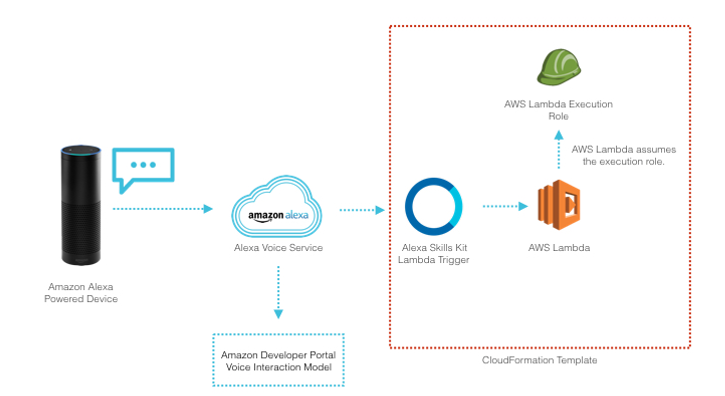
\includegraphics[width=\linewidth]{architecture.png}
  \caption{Project Architecture}
  \label{fig:projectarchitecture}
\end{figure}

Setting up the project was the hardest part of the project and much harder than we initially thought. Setting up the project involved lots of moving parts that needed to connect together and communicate from top to bottom. The project architecture involved four major parts which we will discuss in more details below. 

\section{Alexa Developer Console}
The Alexa Developer Console is where Alexa intents are stored along with the intent slots and slot types. Intents act like traditional function with slots acting as the variables part of the function. Slot types are similar to variable types where you can tell Alexa this slot (variable) is a number. This will ensure when Alexa hears 'what is one plus two' she will instead hear what is 'what is 1 plus 2', 1 and 2 being the two logs given to the function. There are many slot types for a variety of use cases such as German cities, celebrities and video games. Using these slot types Alexa will try match what the user said as best as Alexa can do a value in the given slot type.

\section{AWS Lambda}
AWS Lambda is an event-driven, server-less computing platform provided by Amazon. It saves on resources from traditional server platforms by not running at all times.
AWS Lambda will only run when the application that it is hosting is called. This saves on resources which could be very expensive for start up companies and hobby projects. AWS Lambda integrates extremely well with the Alexa Developer Console because of native support for the Lambda ARN (Amazon Resource Name) which acts as a unique link the the AWS Lambda function

\section{Project Code}
The project code is hosted on AWS Lambda which interacts with the Alexa Developer Console. The skill was programmed in Node.js.  Node.js is an open-source, cross-platform JavaScript run-time environment that executes JavaScript code outside of a browser. Node.js has great integration with AWS Lambda as it was one of the first languages supported by AWS Lambda. We picked Node.js over other languages supported by AWS Lambda because we had a bit of experience with it and we knew with the help of the NPM (Node Package Manager) we could quickly get the application to connect to the API. 

\section{GiantBomb API}
GiantBomb is an American video game website and wiki database that includes data pertaining to video games.

The GiantBomb API required a bit of setup to get working in a basic format. The API required a key which is attached to each request in order for GiantBomb to track any abuse and terminate accounts that abuse the API. We also had to add a 'device' to the HTTP request header in order for GiantBomb to track the application you are making with the API. We added the user GameFinder to the HTTP request in order to use the API by GiantBombs guidelines.









